% This program can be redistributed and/or modified under the terms
% of the GNU Public License, version 3.
%
% Seth Brown, Ph.D.
% sethbrown@drbunsen.org
%
% Compiled with XeLaTeX
% Dependencies:
%   Fontin Sans font (http://www.exljbris.com/fontinsans.html)
%

% TODO: Add citations as bibtex

\documentclass[unknownkeysallowed]{beamer}

\usepackage{graphicx} % graphics
\usepackage{epsfig} % eps graphics
\usepackage{hyperref} % urls
\usepackage{booktabs, caption} % table styling

% suppress navigation bar
\beamertemplatenavigationsymbolsempty

\mode<presentation>
{
  \usetheme{bunsen}
  \setbeamercovered{transparent}
  \setbeamertemplate{items}[circle]
}

% set fonts
\usepackage{fontspec}
\setsansfont{Fontin Sans}
\setbeamerfont{frametitle}{size=\LARGE,series=\bfseries}

% color definitions
\usepackage{color}
\definecolor{uipoppy}{RGB}{225, 64, 5}
\definecolor{uipaleblue}{RGB}{96,123,139}
\definecolor{uiblack}{RGB}{0, 0, 0}

% caption styling
\DeclareCaptionFont{uiblack}{\color{uiblack}}
\DeclareCaptionFont{uipoppy}{\color{uipoppy}}
\captionsetup{labelfont={uipoppy},textfont=uiblack}

% see the macros.tex file for definitions
% This program can be redistributed and/or modified under the terms
% of the GNU Public License, version 3.

% adds reference to bottom right of corner of a slide
\usepackage[absolute,overlay]{textpos} % text references in slide corners
\newcommand\textref[1]{%
  \begin{textblock*}{\paperwidth}(0pt,0.99\textheight)
  \raggedleft \tiny{\emph{#1}}\hspace{.5em}
  \end{textblock*}}

% for drawing circles around numbers
% ex. \circled{1} Add some text here.
\usepackage{tikz}
\newcommand*\circled[1]{\tikz[baseline=(char.base)]{
            \node[shape=circle,draw,inner sep=2pt] (char) {#1};}}


% title slide definition
% TODO: Change image to something less creepy - complex knot pattern?
\title{Get Git}
\author{Chris Keefe, Anthony Simard, Carter Taylor}
\institute{Northern Arizona University \\
Department of Computer Science \\
School of Informatics, Computing, and Cyber Systems \\
}

\date{\today}

%--------------------------------------------------------------------
%                           Introduction
%--------------------------------------------------------------------

\begin{document}

\section{Introduction}
\setbeamertemplate{background}
{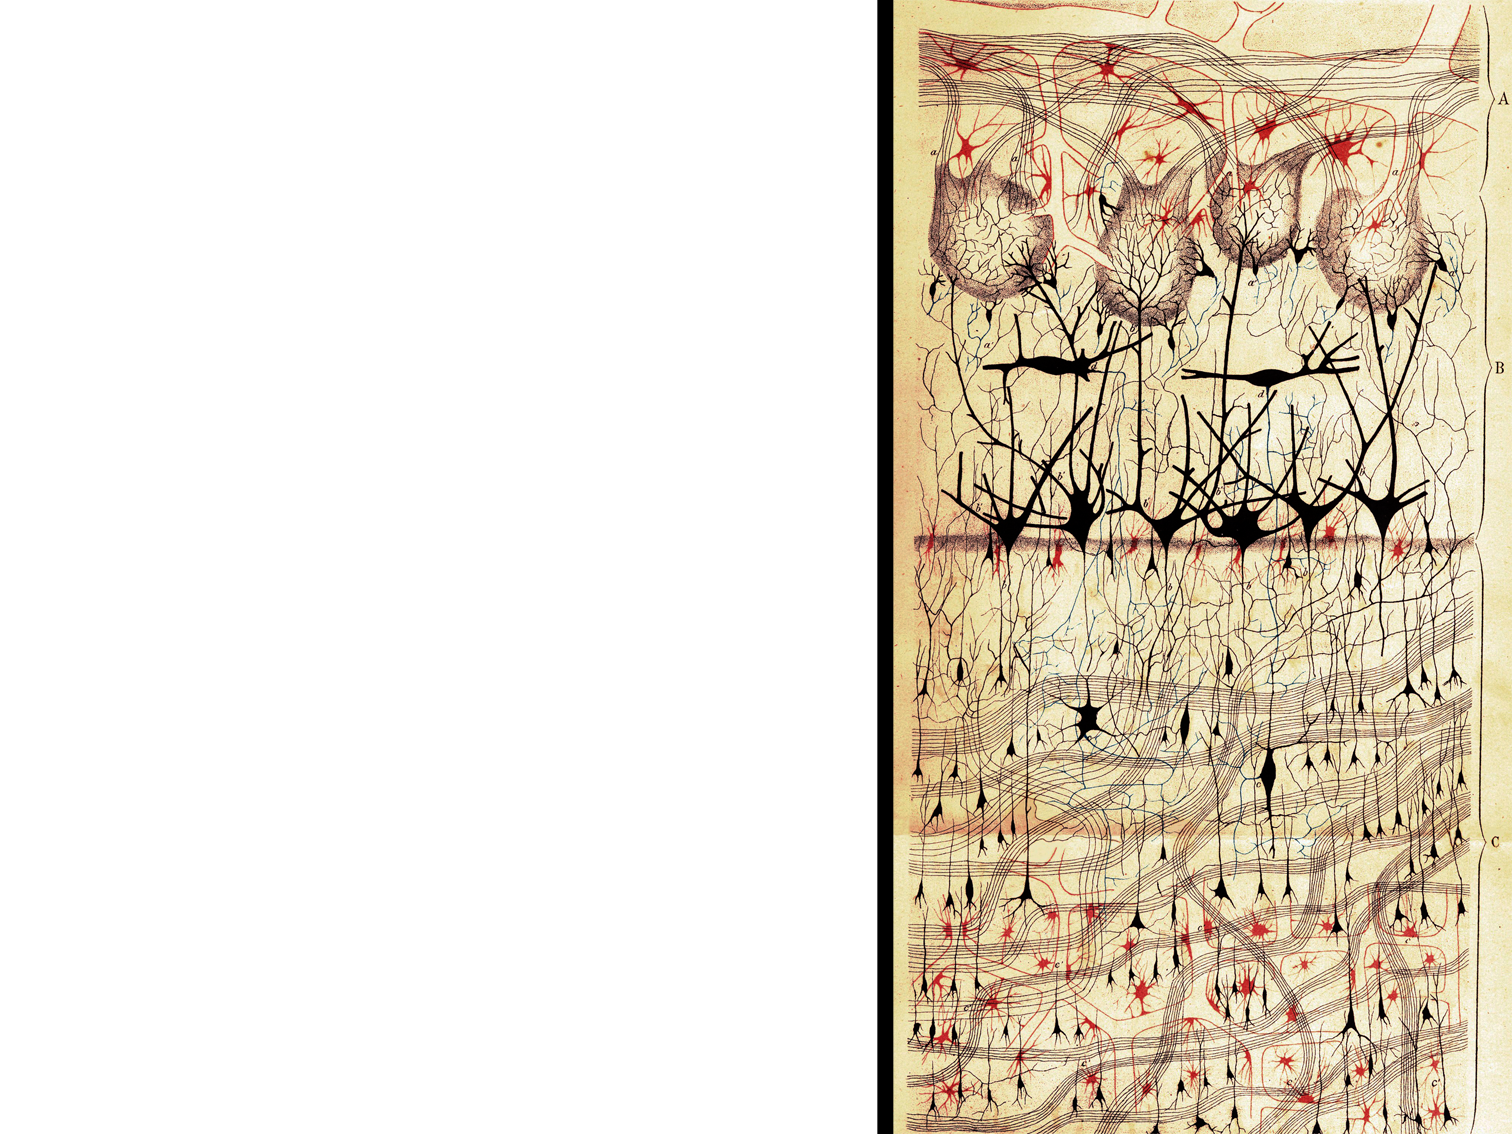
\includegraphics[width=\paperwidth,height=\paperheight]{assets/frontpage_bg}}
\setbeamertemplate{footline}[default]

\begin{frame}
\vspace{2cm}
\begin{columns}
\column{2.75in}
  \titlepage
  \vspace{10cm}
\column{2.0in}
\end{columns}
\end{frame}

%-------------------------------------------------------------------
%                          Section 1
%-------------------------------------------------------------------
%
% Set the background for the rest of the slides.
% Insert infoline
\setbeamertemplate{background}
{
\includegraphics[width=\paperwidth,height=\paperheight]{assets/slide_bg}}
\setbeamertemplate{footline}[bunsentheme]

\section{Getting Started With Git}
\begin{frame}
    \frametitle{Installing Git}
    Packages available from: https://git-scm.com/downloads
    \begin{itemize}
        \item{Windows: Install gitbash.}
        \item{Linux: Install through package manager.}
        \item{Mac: Download git-osx-installer and run. }
    \end{itemize}
    Specific projects may have additional dependencies. Always check the Readme. 
    \vspace{1cm} % generate some space between title and content
\end{frame}


\section{What, Why, and How?}
\begin{frame}
    \frametitle{Git is not GitHub}
    \vspace{0.5cm} % generate some space between title and content
    Git is a powerful version control system
            \begin{itemize}
                \item{Git allows multiple people to easily update the same source}
                \item{Git makes keeping track of changes easy and robust}
       		\item{Git allows people around the world to collaborate on open and closed source projects}
            \end{itemize}
    \vspace{0.5cm}
    GitHub is a site hosting some git repositories
            \begin{itemize}
		\item{It is free to host open source repos. Small private repos too.}
                \item{Large closed-source repos cost \$\$\$}
        	\item{GitHub provides communication and project management tools}
	        \begin{itemize}
		    \item{Pull requests}
		    \item{Issue tracking}
		    \item{Project management}
		    \item{Acess permissioning}
		\end{itemize}
	\item{Git repos absolutely do not need to be on GitHub}
    \end{itemize}
\end{frame}

\begin{frame}
    \frametitle{Some neat repos}
    Check these out:
    \begin{itemize}
        \item{Flight Rules for Git: https://github.com/k88hudson/git-flight-rules}
        \item{Visual Studio Code: https://github.com/Microsoft/vscode}
        \item{Dungeon Crawl Stone Soup: https://github.com/crawl/crawl}
        \item{Tensorflow: https://github.com/tensorflow/tensorflow}
        \item{freeCodeCamp: https://github.com/freeCodeCamp/freeCodeCamp}
        \item{Bootstrap: https://github.com/twbs/bootstrap}
        \item{TheAlgorithms: https://github.com/TheAlgorithms/Python}
    \end{itemize}
    \vspace{1cm} % generate some space between title and content
\end{frame}

\begin{frame}
    \frametitle{Who uses git?}
    \vspace{.5cm}
        \begin{figure}
            \minipage{0.25\textwidth}
                \begin{center}
                    
\includegraphics[width = .4\linewidth]{assets/logos/microsoft_logo}
                \end{center}
            \endminipage
            \minipage{0.25\textwidth}
                \begin{center}
                    
\includegraphics[width = .4\linewidth]{assets/logos/amazon_logo}
                \end{center}
            \endminipage
            \minipage{0.25\textwidth}
                \begin{center}
                    
\includegraphics[width = .4\linewidth]{assets/logos/apple_logo}
                \end{center}
            \endminipage
            \minipage{0.25\textwidth}
                \begin{center}
                    
\includegraphics[width = .4\linewidth]{assets/logos/facebook_logo}
                \end{center}
            \endminipage
        \end{figure}
    \begin{itemize}
        \item{Everyone uses git}
            \begin{itemize}
                \item{Major corporations}
                \item{Governments}
                \item{Independent software developers}
                \item{Students collaborating on projects}
                \item{Many MANY open source projects}
           \end{itemize}
        \item{Git can easily be used for open or closed source projects making it a diverse and powerful tool}
        \item{We used git and GitHub as version control for this presentation}
    \end{itemize}
    \vspace{1cm} % generate some space between title and content
\end{frame}

\begin{frame}
    \frametitle{Why use git?}
    \begin{itemize}
        \item{Employers use version control}
        \item{Collaborations are easier with git}
        \item{Alongside GitHub, Git makes showing off easy}
	\item{Fast, free, redundant version control for your own code}
        \item{It makes contributing to open source much easier.}
    \end{itemize}
    \vspace{1cm} % generate some space between title and content
\end{frame}

\section{Some Vocabulary}
\begin{frame}
	\frametitle{Repository: A fancy bucket}
        \vspace{1cm} % generate some space between title and content
	\begin{itemize}
	    \item{Repositories can be on your local computer, a friend's machine, or on the cloud.}
	    \item{Git repositories hold special hidden files that describe your project's history}
	    \item{You can perform `git` commands from within a repository}
	\end{itemize}
\end{frame}

\begin{frame}
	\frametitle{Commit: the basic unit of change}
        \vspace{1cm} % generate some space between title and content
	\begin{itemize}
	    \item{A commit is a thematically grouped set of changes}
        \vspace{0.5cm} % generate some space between title and content
	    \item{Commits let us understand and manipulate our development history}
        \vspace{0.5cm} % generate some space between title and content
	    \item{Group and name your commits well, so they're easy to work with.}
	\end{itemize}
\end{frame}

\begin{frame}[fragile]
	\frametitle{Branch: development history}
	A is a commit, with a really bad name.

\begin{verbatim}



A  
o



\end{verbatim}
\end{frame}

\begin{frame}[fragile]
	\frametitle{Branch: development history}
	Your software project grows across time.
\begin{verbatim}



A  
o



\end{verbatim}
\end{frame}

\begin{frame}[fragile]
	\frametitle{Branch: development history}
	    Your software project grows across time.
\begin{verbatim}



A  B
o--o
   


\end{verbatim}
\end{frame}

\begin{frame}[fragile]
	\frametitle{Branch: development history}
	    Your software project grows across time.
\begin{verbatim}



A  B  C
o--o--o
      
     
    
\end{verbatim}
\end{frame}

\begin{frame}[fragile]
	\frametitle{Branch: development history}
	You develop many features on your project's branches.
\begin{verbatim}



A  B  C  
o--o--o--\
          \ 
           \--o
              D
\end{verbatim}
\end{frame}

\begin{frame}[fragile]
	\frametitle{Branch: development history}
	You develop many features on your projects branches.
\begin{verbatim}

             
              
A  B  C     E
o--o--o--\--o
          \ 
           \--o
              D  
\end{verbatim}
\end{frame}

\begin{frame}[fragile]
	\frametitle{Branch: development history}
	You develop many features on your projects branches.
\begin{verbatim}
                   F
                /--o
               /
A  B  C     E /
o--o--o--\--o/
          \ 
           \--o
              D  
\end{verbatim}
\end{frame}

\begin{frame}[fragile]
	\frametitle{Branch: development history}
	You develop many features on your projects branches.
\begin{verbatim}
                   F
                /--o
               /
A  B  C     E /  G
o--o--o--\--o/---o
          \ 
           \--o
              D  
\end{verbatim}
\end{frame}

\begin{frame}[fragile]
	\frametitle{Branch: development history}
	You develop many features on your projects branches.
\begin{verbatim}
                   F
                /--o
               /
A  B  C     E /  G
o--o--o--\--o/---o
          \ 
           \--o--o--\
              D  H   \
                      \--o
                        DUMB
\end{verbatim}
\end{frame}

\begin{frame}[fragile]
	\frametitle{Branch: development history}
	You develop many features on your projects branches.
\begin{verbatim}
                   F
                /--o
               /
A  B  C     E /  G
o--o--o--\--o/---o
          \            
           \--o--o--\--o
              D  H   \ I
                      \--o
                        DUMB
\end{verbatim}
\end{frame}

\begin{frame}[fragile]
	\frametitle{Branch: development history}
	When harvest time comes, you pick the good ones and leave the bad.
\begin{verbatim}
                   F
                /--o
               /
A  B  C     E /  G
o--o--o--\--o/---o
          \            
           \--o--o--\--o
              D  H   \ I
                      \--o
                        DUMB
\end{verbatim}
\end{frame}

\begin{frame}[fragile]
	\frametitle{Branch: development history}
	When harvest time comes, you pick the good ones and leave the bad.
\begin{verbatim}
                   F
                /--o
               /
A  B  C     E /  G  F
o--o--o--\--o/---o--o
          \            
           \--o--o--\--o
              D  H   \ I
                      \--o
                        DUMB
\end{verbatim}
\end{frame}

\begin{frame}[fragile]
	\frametitle{Branch: development history}
	When harvest time comes, you pick the good ones and leave the bad.
\begin{verbatim}
                   F
                /--o
               /
A  B  C     E /  G  F      D  H  I  J(merged)
o--o--o--\--o/---o--o-----/o--o--o--o
          \              /
           \--o--o--\--o/
              D  H   \ I
                      \--o
                        DUMB
\end{verbatim}
\end{frame}

\begin{frame}[fragile]
	\frametitle{Branch: development history}
	It's possible to clean up unused branches at any time.
\begin{verbatim}
                   F
                /--o
               /
A  B  C     E /  G  F      D  H  I  J(merged)
o--o--o--\--o/---o--o-----/o--o--o--o
          \              /
           \--o--o--\--o/
              D  H   \ I
                      \--o
                        DUMB
\end{verbatim}
\end{frame}

\begin{frame}[fragile]
	\frametitle{Branch: development history}
	It's possible to clean up unused branches at any time.
\begin{verbatim}
                   F
                /--o
               /
A  B  C     E /  G  F      D  H  I  J(merged)
o--o--o--\--o/---o--o-----/o--o--o--o
          \              /
           \--o--o-----o/
              D  H    I
                      
\end{verbatim}
\end{frame}

\begin{frame}[fragile]
	\frametitle{Branch: development history}
	It's possible to clean up unused branches at any time.
\begin{verbatim}
                   
                
               
A  B  C     E    G  F      D  H  I  J(merged)
o--o--o--\--o----o--o-----/o--o--o--o
          \              /
           \--o--o-----o/
              D  H    I
                      
\end{verbatim}
\end{frame}

\begin{frame}[fragile]
	\frametitle{Branch: development history}
	It's possible to clean up unused branches at any time.
\begin{verbatim}
                   
                
               
A  B  C     E    G  F      D  H  I  J(merged)
o--o--o-----o----o--o------o--o--o--o
          
          
          
                      
\end{verbatim}
\end{frame}

\begin{frame}
    \frametitle{The Master Branch is Sacred}
    "There's only one rule: anything in the master branch is always deployable."
    \begin{itemize}
        \item{Project-wide: The product can always ship. You always have a reservoir of clean code to pull from.}
        \item{Locally: Prevents merge conflicts by ensuring you always have a clean copy to branch from.}
        \item{origin repo vs upstream repo}
    \end{itemize}
    \vspace{1cm} % generate some space between title and content
\end{frame}

% My super roughed up workflow is still there for now just so that slide has something
\setbeamertemplate{background}
{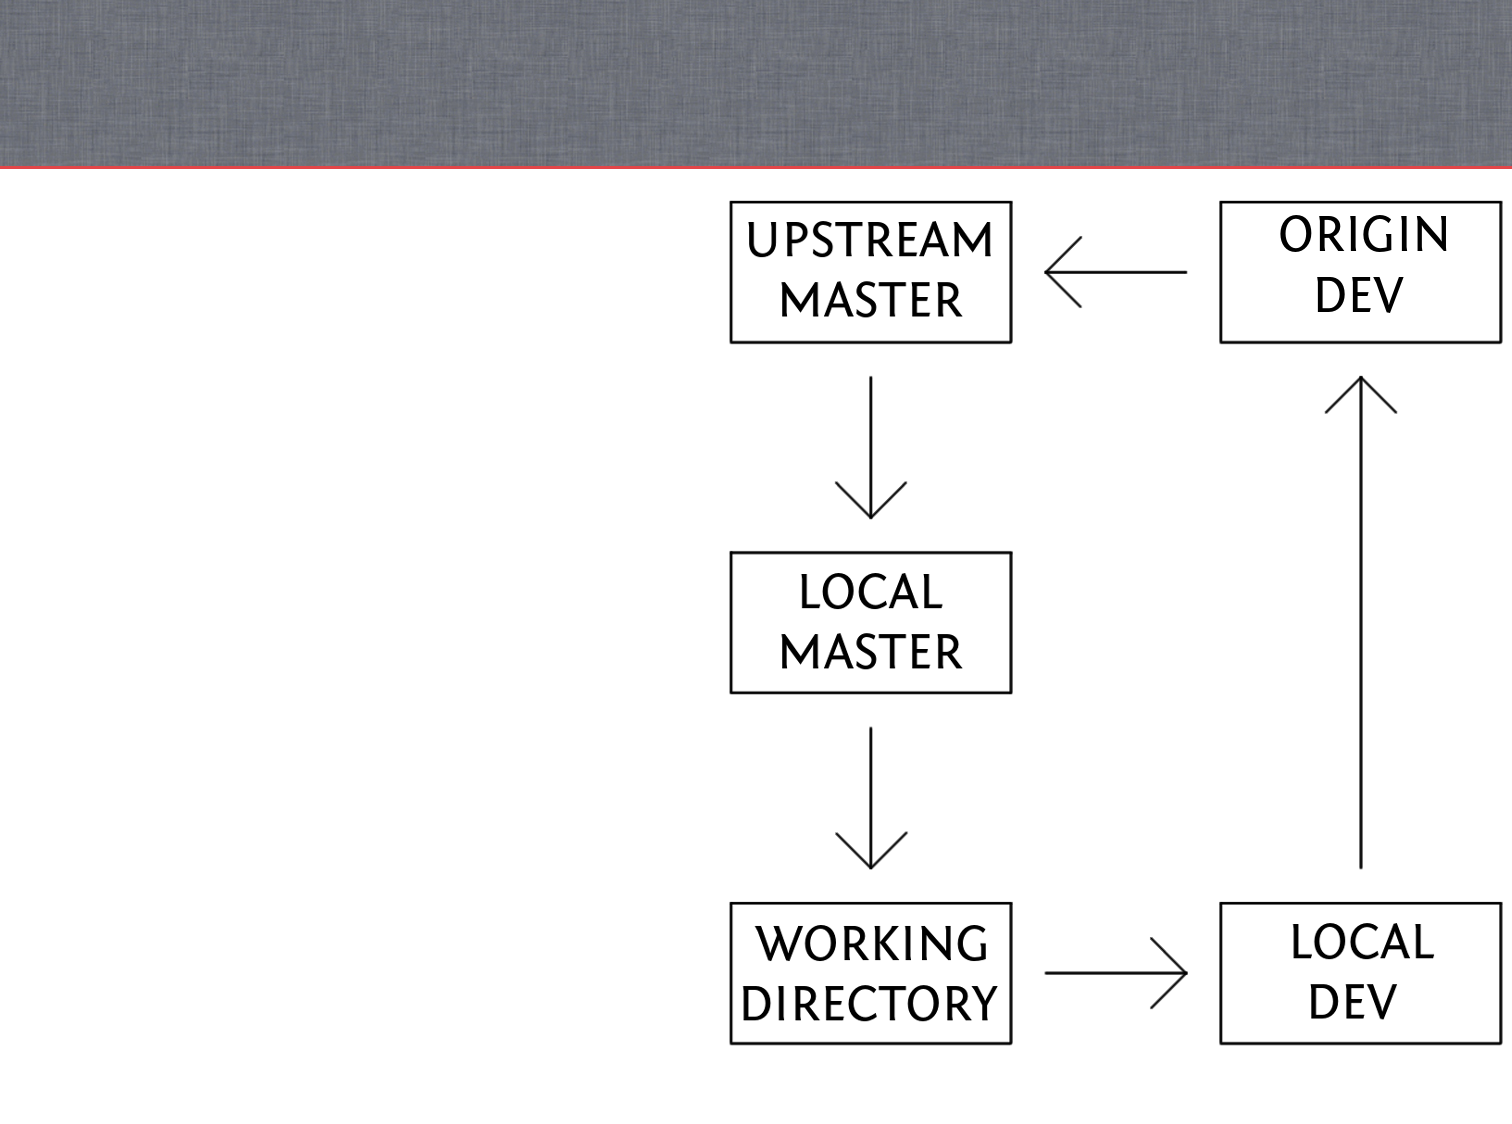
\includegraphics[width=\paperwidth,height=\paperheight]{assets/workflow_bg}}
\begin{frame}
    \vspace{1cm} % generate some space between title and content
    \frametitle{Our Sample Workflow}
        1. Pull from Upstream Master to \\
        Local Master \linebreak\linebreak
        2. Branch to Working Directory \linebreak\linebreak
        3. Make and test changes \linebreak\linebreak
        4. Commit to Local Dev \linebreak\linebreak
        5. Push to Origin Dev \linebreak\linebreak
        6. Open pull request to Upstream \\
        Master
    \vspace{1cm} % generate some space between title and content
\end{frame}
\setbeamertemplate{background}
{
\includegraphics[width=\paperwidth,height=\paperheight]{assets/slide_bg}}

\begin{frame}
    \frametitle{Get source code}
    \begin{itemize}
        \item{Note: For this example, we will be working on an existing repo. For your own projects, it's easy to initialize a new repo. Google "git init".}
        \item{Note: during the presentation, define forking, and note that it is a github, not git process.}
        \item{Fork the repo to which you want to contribute - this creates a complete copy of the repository in the cloud, to which you have edit access.}
        \item{Clone your fork - this copies it to your local machine, where you can work with it.  ``` git clone <paste repo url>```}
    \end{itemize}
    \vspace{1cm} % generate some space between title and content
\end{frame}

\begin{frame}
    \frametitle{Explore and make Changes}
    \begin{itemize}
        \item{Navigate into the repo. ```cd <repo-name>``` You'll see:}
            \begin{itemize}
              \item{source files}
              \item{utility files, including a README and license}
              \item{a hidden .git folder, where the magic lives}
            \end{itemize}
        \item{```git status``` what changes have been made in your repo?}
        \item{```git log``` - what does your commit history look like?}
        \item{```git branch``` - what branch have I checked out?}
        \item{```git remote -v``` - what remote copies of the repo does my git know about?}
    \end{itemize}
    \vspace{1cm} % generate some space between title and content
\end{frame}

\begin{frame}
    \frametitle{Make Changes, and Commit Them}
    \begin{itemize}
        \item{```git checkout -b <branchName>``` - this creates and checks out a new branch, keeping your 'master' clean}
        \item{Edit with your preferred editor. Make changes. Save them.}
        \item{Return to the command line, and git status}
        \item{```git add <filenames>``` tells git which files to track in this commit.}
        \item{```git commit -m 'describes the content of the current commit'``` git saves a record of this point in history to your local machine.}
    \end{itemize}
    \vspace{1cm} % generate some space between title and content
\end{frame}

\begin{frame}
    \frametitle{Push to your Fork}
    \begin{itemize}
        \item{```git push <repo-name> <branch-name>``` - pushes your changes to another repository }
        \item{Git is decentralized. Push can send update any repo to which you have edit access.}
        \item{Your changes may now be public. Consider others before rewriting history.}
    \end{itemize}
    \vspace{1cm} % generate some space between title and content
\end{frame}

\begin{frame}
    \frametitle{Open a Pull Request}
    \begin{itemize}
        \item{Pull requests let the owner of the repository incorporate your branch into their codebase}
        \item{Note: A pull request will merge all new commits on the branch.}
        \item{Be sure to follow the contribution guidelines of the repo owner.}
        \item{Expect constructive criticism and requests for code changes.}
    \end{itemize}
    \vspace{1cm} % generate some space between title and content
\end{frame}

\section{Things to Look Forward To!}
\begin{frame}
    \frametitle{Uh-oh!}
    \begin{itemize}
        \item{TREE DIAGRAM}
        \item{You forgot to create a new branch from master}
        \begin{itemize}
            \item{stash your changes, checkout a new branch, stash pop your changes on the new branch}
            \item{If you've already made multiple commits to master, your process will be more complicated.}
        \end{itemize}
        \item{You forgot to update your source before editing}
        \begin{itemize}
            \item{stash or commit your changes, checkout master, pull code from upstream, merge that code with your working branch, stash pop if necessary}
        \end{itemize}
        \item{You pushed the wrong thing to your fork}
        \begin{itemize}
            \item{if anyone else is using that code, make changes as new commits}
            \item{If you're sure you're the only user, it's possible to "force push" changes to the repo}
        \end{itemize}
        \item{You made a horrible, tangled mess of your commit history}
        \begin{itemize}
            \item{Breathe. Use git's fancy log options, or a GUI to visualize our mess.}
            \item{Don't panic. Draw diagrams, and get clear on what needs to happen. Google is your friend.}
            \item{Go for a walk, and come back to it. Git stores all kinds of information on your repo - even "irreversible" damage can usually be fixed with the help of ```git reflog```}
        \end{itemize}
    \end{itemize}
    \vspace{1cm} % generate some space between title and content
\end{frame}

\begin{frame}
    \frametitle{On the bright side...}
    \begin{itemize}
        \item{You'll never lose committed changes.}
        \item{You have fine-grained control over your codebase and its history}
        \item{Sharing your work with collaborators and possible employers is super easy.}
        \item{Editing your code on different machines is super easy}
        \item{You can contribute effectively to all kinds of amazing projects.}
    \end{itemize}
    \vspace{1cm} % generate some space between title and content
\end{frame}

\section{Let's do this!}
\begin{frame}
    \frametitle{Project Overview}
    Goals:
    \begin{itemize}
        \item{numerical list?}
        \item{Contribute unique content pages to a web site.}
        \item{Edit existing pages in a workflow structured to avoid conflict.}
        \item{Break things, while editing existing pages without coordination.}
        \item{Set low expectations, exceed them, and have fun!}
    \end{itemize}
    Format:
    \begin{itemize}
        \item{Everyone with a laptop with git installed and a github profile signs up.}
        \item{All others assigned at random to a group}
        \item{More-experienced users are encouraged to help troubleshoot.}
    \end{itemize}
    \vspace{1cm} % generate some space between title and content
\end{frame}

\begin{frame}
\frametitle{Git Cheat Sheet}
\begin{columns}
    \column{2.75in}
        \begin{itemize}
            \item{```git init```}
            \item{```git clone <repo url>```}
            \item{```git fetch <remote alias>```}
            \item{```git pull <remote alias> <branch>```}
            \item{```git checkout <branch name>```}
            \item{```git checkout -b <branch name>```}
            \item{```git push <remote alias> <branch>```}

        \end{itemize}
    \column{2.0in}
        \begin{itemize}
            \item{```git status```}
            \item{```git git log```}
            \item{```git branch```}
            \item{```git remote -v```}
            \item{```git add <filename>```}
            \item{```git commit -m 'message'```}
        \end{itemize}
    \end{columns}
    \vspace{1cm} % generate some space between title and content
\end{frame}

\end{document}
